\documentclass[11pt,a4paper]{article}
\usepackage[utf8]{inputenc}
\usepackage[T1]{fontenc}
\usepackage[spanish,es-noquoting]{babel}
\usepackage{amsmath,amssymb}
\usepackage{graphicx}
\usepackage{booktabs}
\usepackage{float}
\usepackage{listings}
\usepackage{xcolor}
\usepackage{caption}
\usepackage[margin=2.4cm]{geometry}
\usepackage{hyperref}
\hypersetup{colorlinks=true,linkcolor=blue!50!black,urlcolor=blue!50!black}

\definecolor{codegray}{gray}{0.95}
\definecolor{commentgreen}{rgb}{0.0,0.5,0.0}
\definecolor{keywordblue}{rgb}{0.0,0.0,0.6}
\definecolor{stringmauve}{rgb}{0.58,0.0,0.82}
\lstset{
  language=Matlab, basicstyle=\ttfamily\footnotesize,
  backgroundcolor=\color{codegray}, commentstyle=\color{commentgreen}\itshape,
  keywordstyle=\color{keywordblue}\bfseries, stringstyle=\color{stringmauve},
  numbers=left, numberstyle=\tiny\color{gray}, numbersep=6pt,
  frame=single, rulecolor=\color{gray!40}, breaklines=true,
  columns=fullflexible, showstringspaces=false, captionpos=b,
  xleftmargin=14pt, framexleftmargin=14pt
}
\newcommand{\code}[1]{\texttt{\small #1}}

\begin{document}

% ================= DATOS =================
\section{Datos generales}
\begin{center}
\renewcommand{\arraystretch}{1.3}
\begin{tabular}{ll}
\toprule
\textbf{Curso} & Inteligencia Artificial Aplicada al Control (ICA636-0001) \\
\textbf{Trabajo} & Tarea 1 --- Redes Neuronales Estáticas \\
\textbf{Alumno} & Joel Arzapalo Guerra \\
\textbf{Código} & 20032006 \\
\textbf{Fecha} & \today \\
\bottomrule
\end{tabular}
\end{center}
\vspace{0.5cm}

% ================= INTRODUCCION =================
\section{Introducción}
Este trabajo analiza cuatro programas MATLAB que entrenan una \textbf{red neuronal
estática} (red multicapa de una capa oculta) para \textbf{aproximar funciones} a
partir de datos con ruido, mediante \emph{retropropagación del error} (descenso de
gradiente). Todos comparten la misma arquitectura: entrada $\to$ capa oculta ($nm$
neuronas con función de activación no lineal) $\to$ salida lineal, con pesos $v$
(entrada--oculta) y $w$ (oculta--salida) tratados en forma matricial.

Los cuatro scripts ilustran, de forma incremental, los aspectos fundamentales del
entrenamiento:
\begin{itemize}
  \item \code{NeuronLinealPatron.m}: ajuste de una recta ruidosa con entrenamiento
        \emph{patrón} (en línea): los pesos se actualizan tras \emph{cada} muestra.
  \item \code{NeuronLinealPatronBatch.m}: el mismo problema con entrenamiento por
        \emph{lote}: el gradiente se acumula sobre todas las muestras y se
        actualiza una vez por época.
  \item \code{NeuronCubicaEscalamiento.m}: ajuste de una función \emph{cúbica} y estudio
        del \textbf{problema de escalamiento} de la salida.
  \item \code{NeuronDosEntradasDosSalidas.m}: aproximación de \textbf{múltiples entradas
        y múltiples salidas} (2 entradas y 2 salidas).
\end{itemize}
Los comentarios de los scripts proponen explícitamente estudiar el número de neuronas
$nm$, el valor inicial de los pesos, el tipo de activación y la neurona de \emph{sesgo}
(bias). El informe cubre (i) el \textbf{análisis del código} y (ii) los \textbf{resultados
experimentales} sobre esos parámetros. Los scripts (interactivos, con \code{input()}) se
adaptaron a versiones no interactivas y reproducibles (semilla fija), encapsulando el
entrenamiento en la función \code{lib\_mlp.m}, fiel a la formulación original.

% ================= ANALISIS DE CODIGO =================
\section{Análisis del código}

\subsection{Estructura común}
Todos generan datos $\{x_k, y^*_k\}$ (una función objetivo más ruido gaussiano),
inicializan los pesos aleatoriamente y ejecutan el bucle de entrenamiento. La salida de
cada neurona oculta es $n=f(m)$ con $m=v^{\top}\text{in}$, y la salida de la red es
$\text{out}=w^{\top}n$. Las activaciones disponibles (y sus derivadas, necesarias para
la regla de la cadena) son:
\[
  \underbrace{n=\tfrac{1}{1+e^{-m}}}_{\text{logística}},\;
  \underbrace{n=\tfrac{2}{1+e^{-m}}-1}_{\text{bipolar}},\;
  \underbrace{n=e^{-m^2}}_{\text{gaussiana}}.
\]
El costo es $J=\tfrac{1}{2N}\sum_k e_k^2$ con $e=\text{out}-y^*$, y los gradientes son
$\partial J/\partial w = n\,e^{\top}$ y
$\partial J/\partial v = \text{in}\,(f'(m)\odot(w\,e))^{\top}$.

\subsection{Patrón vs lote}
La diferencia esencial entre los dos primeros scripts es \emph{cuándo} se actualizan los
pesos:

\begin{lstlisting}[caption={Entrenamiento PATRON: se actualiza dentro del bucle de muestras.}]
for k = 1:N
  ...  er = out - yb(k,1);
  dJdw = er.*n;   dJdv = er.*in*(w.*dndm)';
  w = w - eta*dJdw;   % actualizacion INMEDIATA (cada muestra)
  v = v - eta*dJdv;
end
\end{lstlisting}

\begin{lstlisting}[caption={Entrenamiento LOTE: se acumula y se actualiza una vez por epoca.}]
for k = 1:N
  ...  dJdw = dJdw + n*er';   dJdv = dJdv + in*(dndm.*(w*er))';
end
w = w - eta*dJdw/N;   % actualizacion tras recorrer TODO el conjunto
v = v - eta*dJdv/N;
\end{lstlisting}

El \textbf{sesgo} (bias) se implementa añadiendo una columna constante a la entrada
(\code{x = [x ones(N,1)]}, \code{ne = ne+1}), lo que da a cada neurona un término
independiente. El criterio de parada usa la mejora relativa porcentual del costo
(\code{dJpor < errorporc}).

\subsection{Escalamiento (cúbica) y salida vectorial (MIMO)}
\code{NeuronCubicaEscalamiento.m} multiplica la salida deseada por un \code{FACTOR} para
estudiar qué pasa cuando su magnitud crece: con tasa de aprendizaje fija, el
entrenamiento se vuelve sensible a la escala de $y^*$. \code{NeuronDosEntradasDosSalidas.m}
generaliza a $ns=2$ salidas: $w$ pasa a ser $nm\times ns$ y el error $e$ es un vector;
la misma regla de la cadena se aplica en bloque. Incluye un factor de pendiente $a$ por
neurona en la sigmoide $n=2/(1+e^{-m/a})-1$.

% ================= RESULTADOS =================
\section{Resultados experimentales}
Resultados con las versiones no interactivas (semilla fija). Las figuras se generan con
\code{Informe/exp/run\_all.m}.

\subsection{Ajuste de una recta: patrón vs lote, bias, $\eta$ e inicialización}
\label{sec:RA}
Se ajustó la recta ruidosa $y=x+2+0.2\,\mathcal{N}$ ($n_m=10$). Ambos modos de
entrenamiento alcanzan el nivel de ruido irreducible ($\sigma=0.2$): RMSE $0.231$ en
modo \textbf{patrón} y $0.256$ en \textbf{lote} (Fig.~\ref{fig:RApb}, ajuste en
Fig.~\ref{fig:RAfit}). El modo patrón converge en menos épocas —actualiza los pesos $N$
veces por época— pero con una trayectoria de costo más ruidosa; el lote es más suave y
estable por época.

\begin{figure}[H]
\centering
\begin{minipage}{0.48\linewidth}\centering
  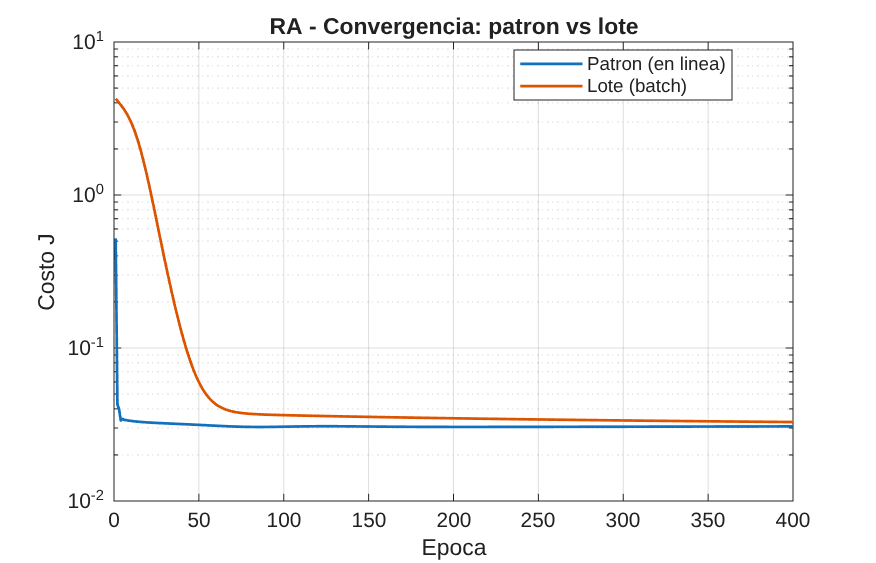
\includegraphics[width=\linewidth]{figs/RA_pattern_batch.png}
  \caption{Convergencia: patrón vs lote.}\label{fig:RApb}
\end{minipage}\hfill
\begin{minipage}{0.48\linewidth}\centering
  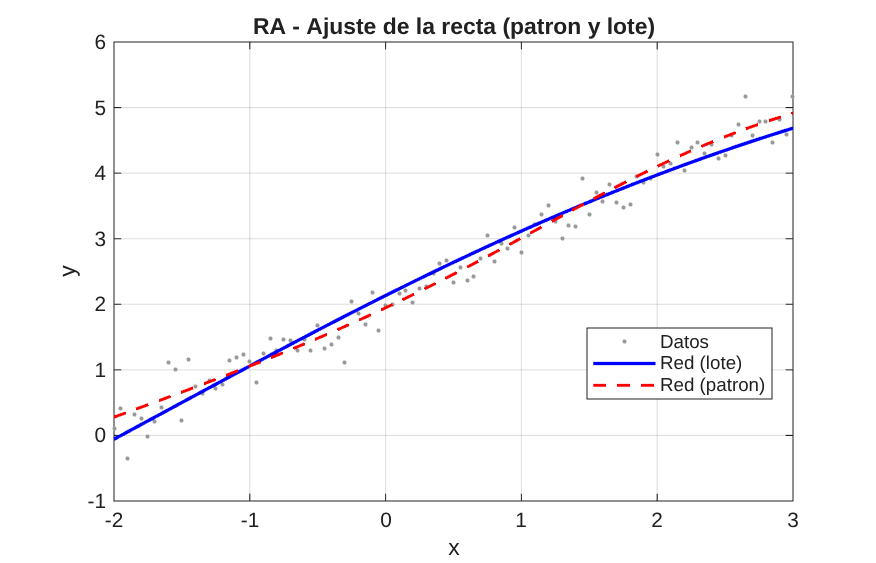
\includegraphics[width=\linewidth]{figs/RA_fit.png}
  \caption{Ajuste de la recta (patrón y lote).}\label{fig:RAfit}
\end{minipage}
\end{figure}

\paragraph{Sesgo.} Es el efecto más marcado: \emph{con} neurona de sesgo el RMSE es
$0.234$, pero \emph{sin} sesgo sube a $1.95$ (Fig.~\ref{fig:RAbias}). Sin el término
independiente la red no puede representar el desplazamiento $b=2$ de la recta (con
activación bipolar, en $x=0$ todas las salidas ocultas valen $0$ y la red solo produce
$0$), por lo que el ajuste falla.

\paragraph{Tasa $\eta$ e inicialización.} La tasa de aprendizaje muestra el compromiso
habitual (Fig.~\ref{fig:RAeta}): $\eta$ pequeño converge lento y $\eta$ grande, rápido
pero con oscilaciones. La escala inicial de los pesos influye poco en el resultado final
(RMSE entre $0.224$ y $0.263$), aunque una inicialización muy grande ($5.0$) empeora
levemente la convergencia (Fig.~\ref{fig:RAinit}).

\begin{figure}[H]
\centering
\begin{minipage}{0.32\linewidth}\centering
  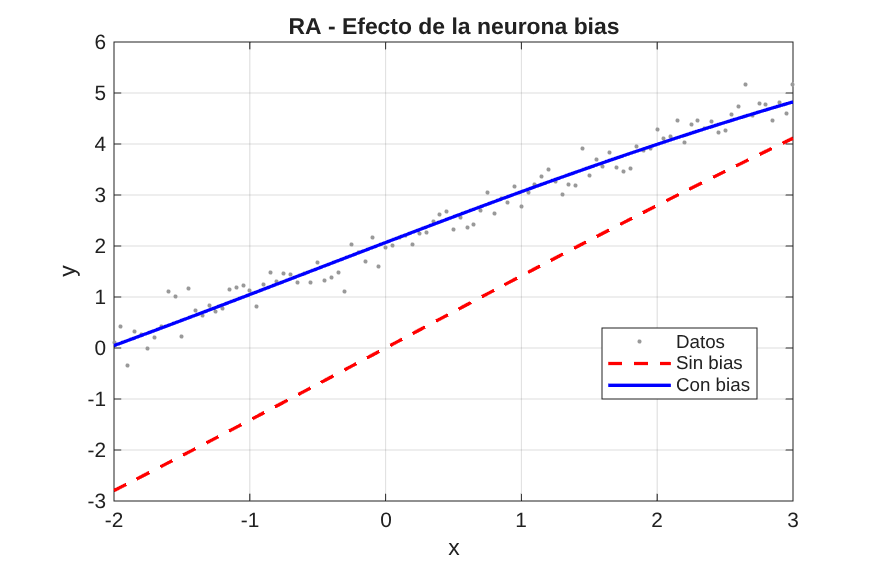
\includegraphics[width=\linewidth]{figs/RA_bias.png}
  \caption{Con y sin sesgo.}\label{fig:RAbias}
\end{minipage}\hfill
\begin{minipage}{0.32\linewidth}\centering
  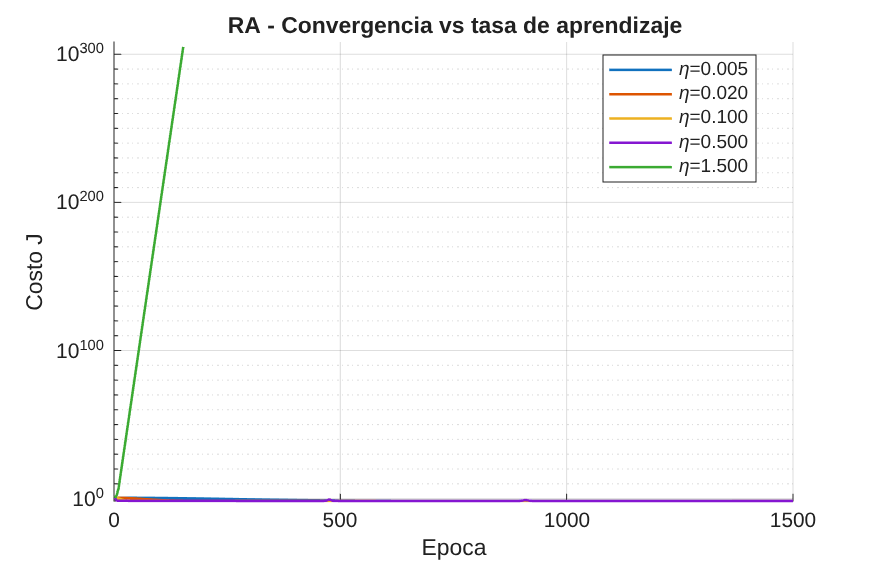
\includegraphics[width=\linewidth]{figs/RA_eta.png}
  \caption{Convergencia vs $\eta$.}\label{fig:RAeta}
\end{minipage}\hfill
\begin{minipage}{0.32\linewidth}\centering
  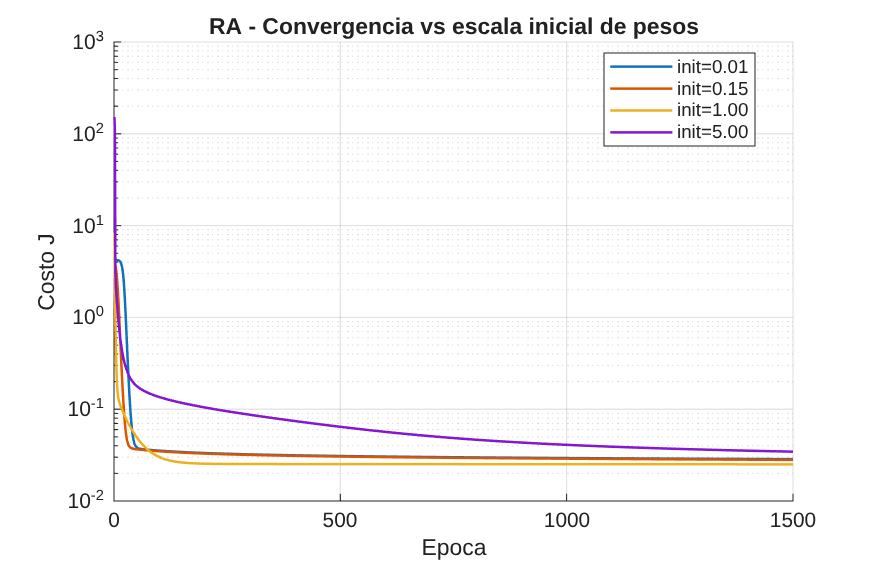
\includegraphics[width=\linewidth]{figs/RA_init.png}
  \caption{Convergencia vs init.}\label{fig:RAinit}
\end{minipage}
\end{figure}

\subsection{Aproximación de una cúbica: neuronas y activación}
\label{sec:RB}
Se aproximó una función cúbica ruidosa. El \textbf{número de neuronas} determina la
capacidad de la red (Tabla~\ref{tab:RB}, Fig.~\ref{fig:RBnm}): con $n_m=1$--$2$ la red
\emph{subajusta} (RMSE $1.19$ y $0.81$), a partir de $n_m=5$ el ajuste alcanza el nivel
de ruido (RMSE $\approx 0.26$) y añadir más neuronas no mejora —incluso empeora
levemente, por la mayor dificultad de entrenar más parámetros en un número fijo de
épocas. La Fig.~\ref{fig:RBfit} contrasta el subajuste ($n_m=2$) con un ajuste adecuado.

\begin{table}[H]\centering
\caption{RMSE del ajuste de la cúbica según el número de neuronas ocultas.}
\label{tab:RB}
\begin{tabular}{lcccccc}
\toprule
$n_m$ & 1 & 2 & 5 & 10 & 25 & 50 \\
RMSE & 1.19 & 0.81 & 0.26 & 0.33 & 0.39 & 0.37 \\
\bottomrule
\end{tabular}
\end{table}

En cuanto a la \textbf{función de activación} (Fig.~\ref{fig:RBact}), las tres logran
ajustar la cúbica; en este problema la gaussiana obtuvo el menor error (RMSE $0.237$),
seguida de la logística ($0.327$) y la bipolar ($0.395$).

\begin{figure}[H]
\centering
\begin{minipage}{0.32\linewidth}\centering
  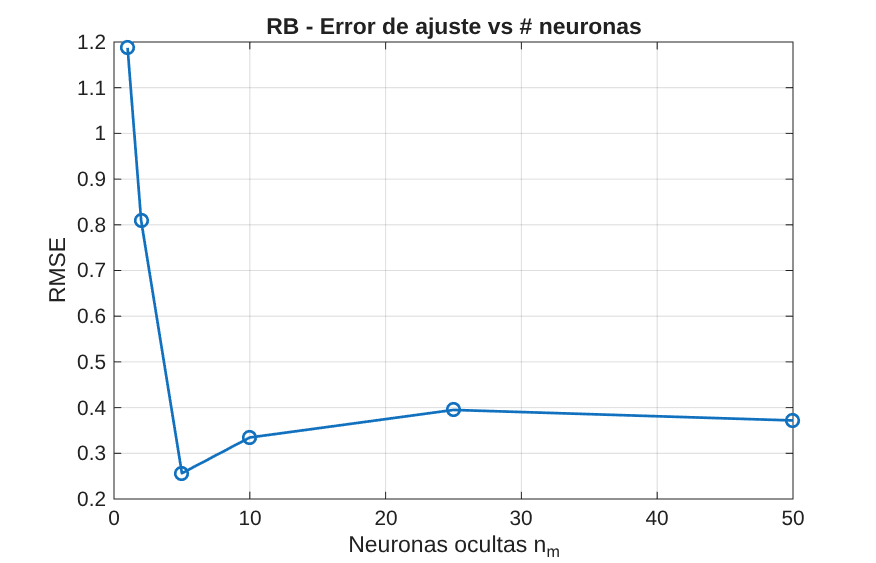
\includegraphics[width=\linewidth]{figs/RB_neurons.png}
  \caption{RMSE vs $n_m$.}\label{fig:RBnm}
\end{minipage}\hfill
\begin{minipage}{0.32\linewidth}\centering
  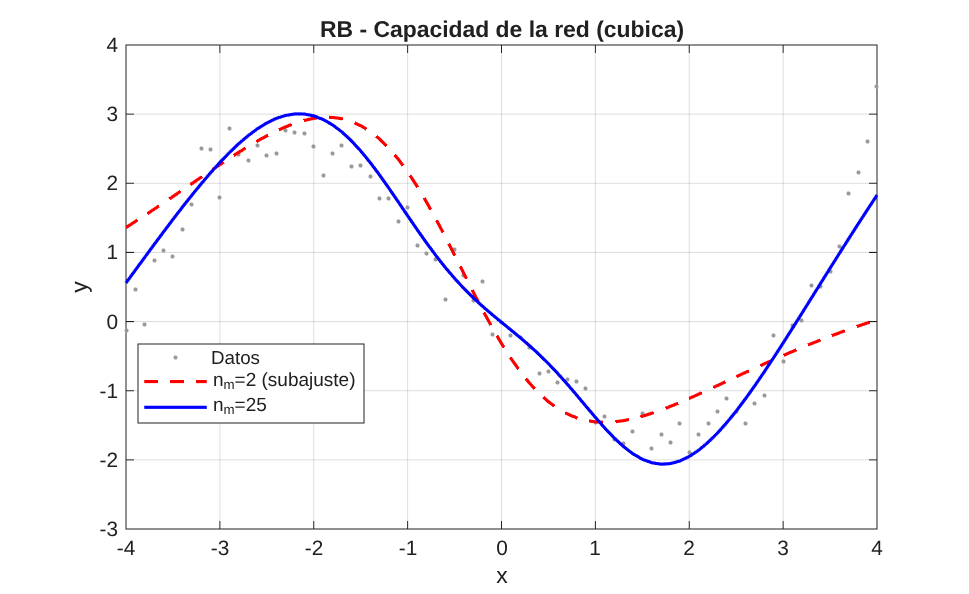
\includegraphics[width=\linewidth]{figs/RB_fit.png}
  \caption{Subajuste vs ajuste.}\label{fig:RBfit}
\end{minipage}\hfill
\begin{minipage}{0.32\linewidth}\centering
  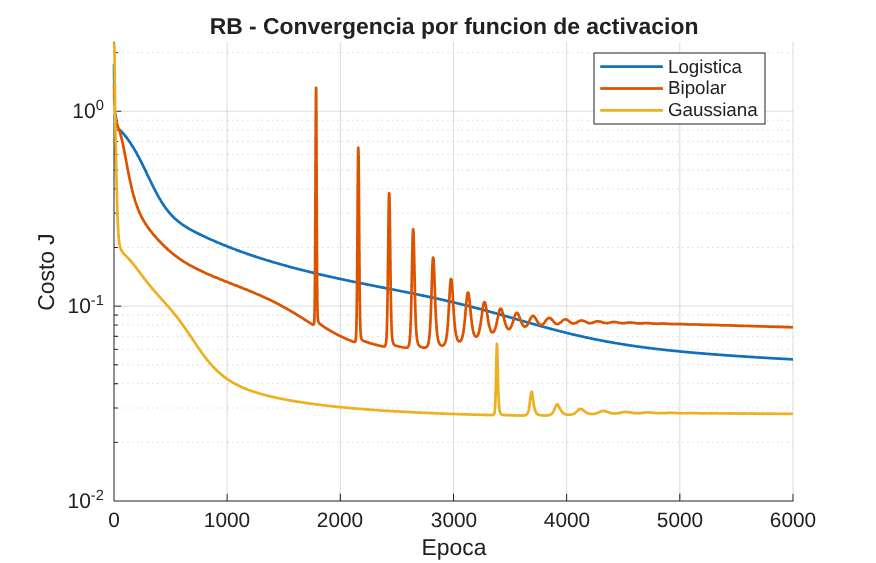
\includegraphics[width=\linewidth]{figs/RB_activation.png}
  \caption{Activación.}\label{fig:RBact}
\end{minipage}
\end{figure}

\subsection{El problema de escalamiento de la salida}
\label{sec:RC}
Se multiplicó la salida deseada por un \code{FACTOR} creciente, entrenando con la
\emph{misma} tasa $\eta=0.1$ en dos variantes: sin escalar la salida, y escalándola a
$\approx[-1,1]$ (para luego devolver la predicción a su escala original). El error se mide contra la señal
\emph{limpia}. El resultado (Tabla~\ref{tab:RC}, Fig.~\ref{fig:RC}) muestra el problema
de escalamiento: \textbf{sin escalar, la calidad del ajuste depende fuertemente de la
magnitud} —de un error relativo de $0.05$ para magnitudes moderadas hasta $0.63$ (ajuste
pobre) para magnitudes grandes, con la misma $\eta$—. \textbf{Escalando la salida el
error es constante ($\approx0.21$) e independiente de la magnitud}: un único $\eta$
funciona para cualquier escala. La lección práctica es \emph{normalizar la salida} (y las
entradas) antes de entrenar, para que la elección de $\eta$ no dependa de las unidades del
problema.

\begin{table}[H]\centering
\caption{Error relativo (vs señal limpia) según la magnitud de la salida y $\eta$ fijo.}
\label{tab:RC}
\begin{tabular}{lccccc}
\toprule
FACTOR & 1 & 10 & 100 & 1000 & 5000 \\
\midrule
Sin escalar & 0.194 & 0.047 & 0.295 & 0.634 & 0.633 \\
Escalada $[-1,1]$ & 0.212 & 0.212 & 0.212 & 0.212 & 0.212 \\
\bottomrule
\end{tabular}
\end{table}

\begin{figure}[H]
\centering
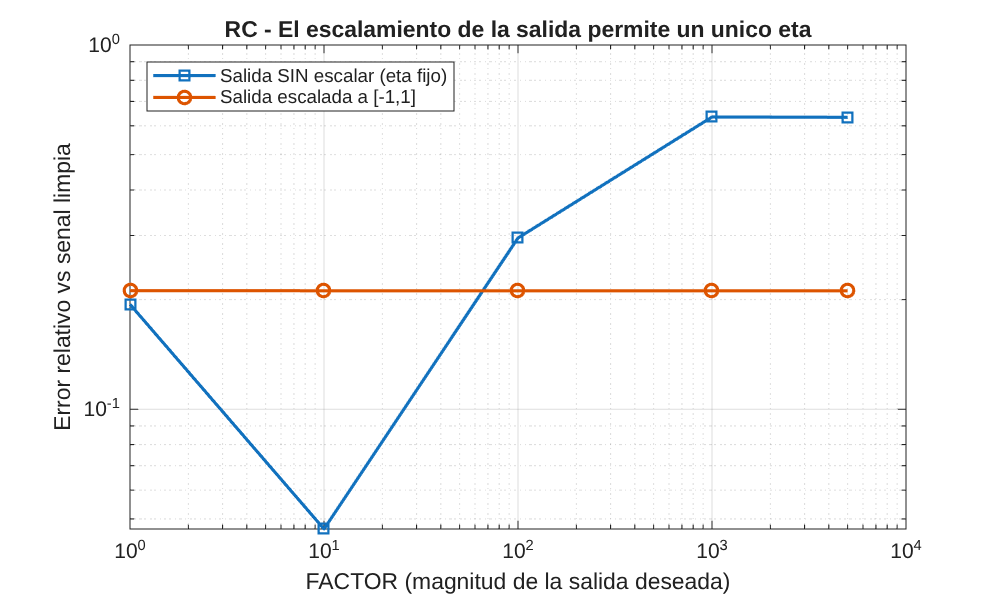
\includegraphics[width=0.6\linewidth]{figs/RC_scaling.png}
\caption{El escalamiento de la salida hace que un único $\eta$ funcione para toda
magnitud (escala log--log).}\label{fig:RC}
\end{figure}

\subsection{Aproximación de múltiples entradas y salidas (2 entradas, 2 salidas)}
\label{sec:RD}
La misma arquitectura se extiende a dos salidas ($w$ pasa a ser $n_m\times2$). Con
$n_m=50$ la red aproxima simultáneamente las dos funciones objetivo con RMSE $0.354$ para
$y_1$ y $0.116$ para $y_2$ (Fig.~\ref{fig:RDmimo}), del orden del ruido añadido a cada
salida. La convergencia (Fig.~\ref{fig:RDconv}) es monótona. Esto confirma que una única
red de una capa oculta puede modelar relaciones de varias entradas y varias salidas.

\begin{figure}[H]
\centering
\begin{minipage}{0.56\linewidth}\centering
  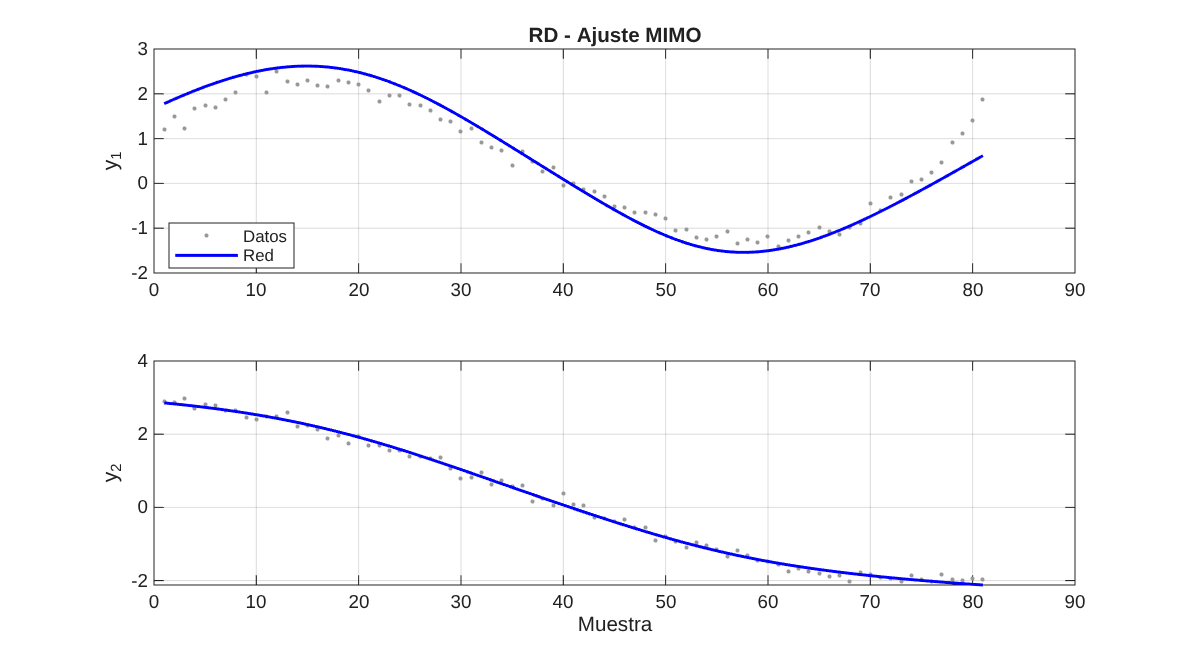
\includegraphics[width=\linewidth]{figs/RD_mimo.png}
  \caption{Ajuste de las dos salidas.}\label{fig:RDmimo}
\end{minipage}\hfill
\begin{minipage}{0.40\linewidth}\centering
  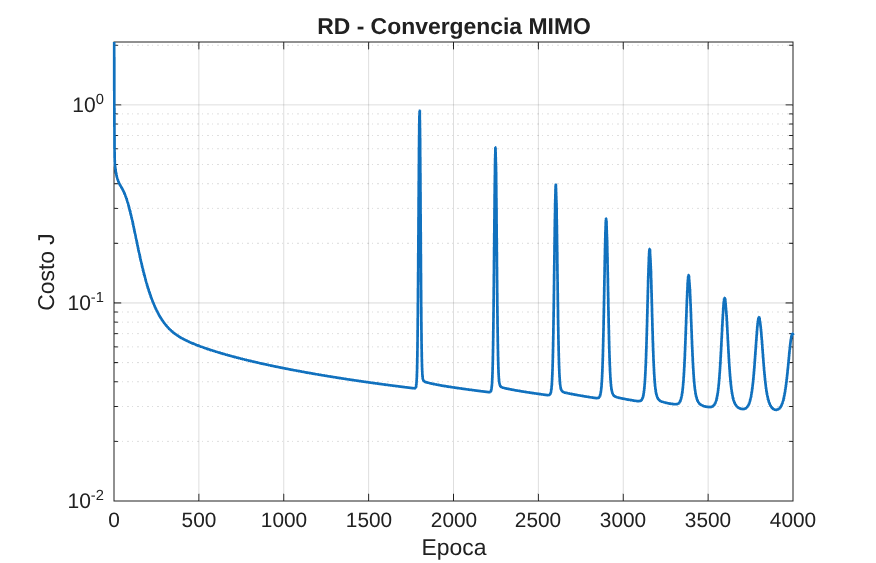
\includegraphics[width=\linewidth]{figs/RD_conv.png}
  \caption{Convergencia (dos salidas).}\label{fig:RDconv}
\end{minipage}
\end{figure}

% ================= CONCLUSIONES =================
\section{Conclusiones}
\begin{enumerate}
  \item \textbf{Patrón vs lote} (Sec.~\ref{sec:RA}): ambos ajustan la recta hasta el nivel
  de ruido; el entrenamiento patrón (en línea) converge en menos épocas pero de forma más
  ruidosa, mientras que el lote es más estable por época.

  \item \textbf{La neurona de sesgo es esencial} para representar desplazamientos: sin ella
  el ajuste de la recta falla (RMSE $1.95$ frente a $0.23$ con sesgo).

  \item \textbf{El número de neuronas fija la capacidad} (Sec.~\ref{sec:RB}): muy pocas
  subajustan; a partir de un umbral ($n_m\!\approx\!5$ para la cúbica) se alcanza el nivel
  de ruido y más neuronas no ayudan (e incluso complican el entrenamiento a épocas fijas).

  \item \textbf{La activación importa poco si hay capacidad suficiente}: las tres
  funciones ensayadas ajustan la cúbica, con diferencias menores de error.

  \item \textbf{El escalamiento es clave} (Sec.~\ref{sec:RC}): sin normalizar la salida,
  el desempeño con una $\eta$ fija depende fuertemente de la magnitud del problema;
  escalando la salida (y las entradas) a un rango normalizado, un mismo $\eta$ funciona
  para cualquier escala. Junto con la elección de $\eta$, es el ajuste práctico más
  importante.

  \item \textbf{La arquitectura admite múltiples salidas} (Sec.~\ref{sec:RD}): una sola red
  de una capa oculta aproxima relaciones de varias entradas y varias salidas.
\end{enumerate}

\appendix
\section{Archivos del proyecto}
Los experimentos se ejecutan con \code{Informe/exp/run\_all.m}. El entrenamiento está
en \code{lib\_mlp.m} (una capa oculta, retropropagación, con modos patrón/lote y
activaciones logística/bipolar/gaussiana). Cada experimento RA--RD guarda sus figuras en
\code{Informe/figs/} y sus métricas en \code{*\_metrics.mat}.

\end{document}
